\documentclass[a4paper,11pt]{article}
\usepackage{graphicx}
\usepackage{url}
\usepackage{amsmath}
\usepackage{amsfonts}
\usepackage{geometry}
\usepackage[numbers]{natbib}
\usepackage{cite}
\usepackage{listings}
\usepackage{hyperref}
\geometry{margin=1in}
\bibliographystyle{plain}
\graphicspath{{../../04-outputs/02-mushroom-edibility-analysis-replication/}}

\title{Replication Study: Mushroom edibility analysis}
\author{}
\date{}

\begin{document}  

\maketitle  

\section*{Abstract}
This study replicates the Random Forest approach from the article ``Edibility Detection of Mushroom Using Ensemble Methods'' by Brital et al.~\citep{brital2019edibility}, originally published in the \textit{International Journal of Image, Graphics and Signal Processing} in 2019. Using a larger and more feature-rich version of the UCI Mushroom dataset, we implemented the analysis in the R environment and evaluated model performance across various train/test splits. In addition to model replication, we conducted visual and statistical feature analysis to interpret what contributes most to accurate classification. Results consistently showed near-perfect prediction accuracy, reinforcing the effectiveness of Random Forests in this application.

\section{Introduction}
Classifying whether a mushroom is edible or poisonous based on observable traits has long been a benchmark problem in machine learning. In their 2019 paper, Brital et al.~\citep{brital2019edibility} explored this task using ensemble methods\textemdash namely Bagging, Boosting, and Random Forest\textemdash and reported high classification performance, with Random Forest yielding the best results. Their work was conducted using a subset of mushroom features and implemented in MATLAB. In this replication, we revisit their Random Forest analysis from a modern data science perspective. We use the R ecosystem, apply the method to a newer, expanded mushroom dataset, and further investigate which features are most informative using both statistical and model-derived metrics. Our goal is not only to replicate performance but also to better understand the model’s behavior through exploratory visualization and feature importance analysis.

\section{Dataset and Preprocessing}
For this study, we used the \href{https://archive.ics.uci.edu/dataset/848/secondary+mushroom+dataset}{UCI Secondary Mushroom Dataset}, which includes 61,069 entries describing mushroom characteristics such as cap diameter, stem shape, gill attachment, and spore print color. Each entry is labeled as either edible (e) or poisonous (p).

The dataset includes a mix of categorical and numerical features. Categorical variables were converted into factor types for modeling purposes, while numerical variables were standardized to improve interpretability and scale consistency. Data was split into training and test subsets using stratified sampling to ensure balanced class representation.


\section{Exploratory Data Analysis}

Before constructing any models, we examined the distributional patterns of both numerical and categorical features to better understand how they relate to mushroom edibility. This initial step serves two purposes: it helps identify potential signal in the data and reveals any irregularities that could affect downstream modeling.

\subsection{Numerical Feature Patterns}

Figure~\ref{fig:violin} presents violin plots overlaid with boxplots for the three numeric attributes: \texttt{cap\_diameter}, \texttt{stem\_height}, and \texttt{stem\_width}. Each plot compares the distribution of a feature across the two classes: edible and poisonous.

\begin{figure}[h]
\centering
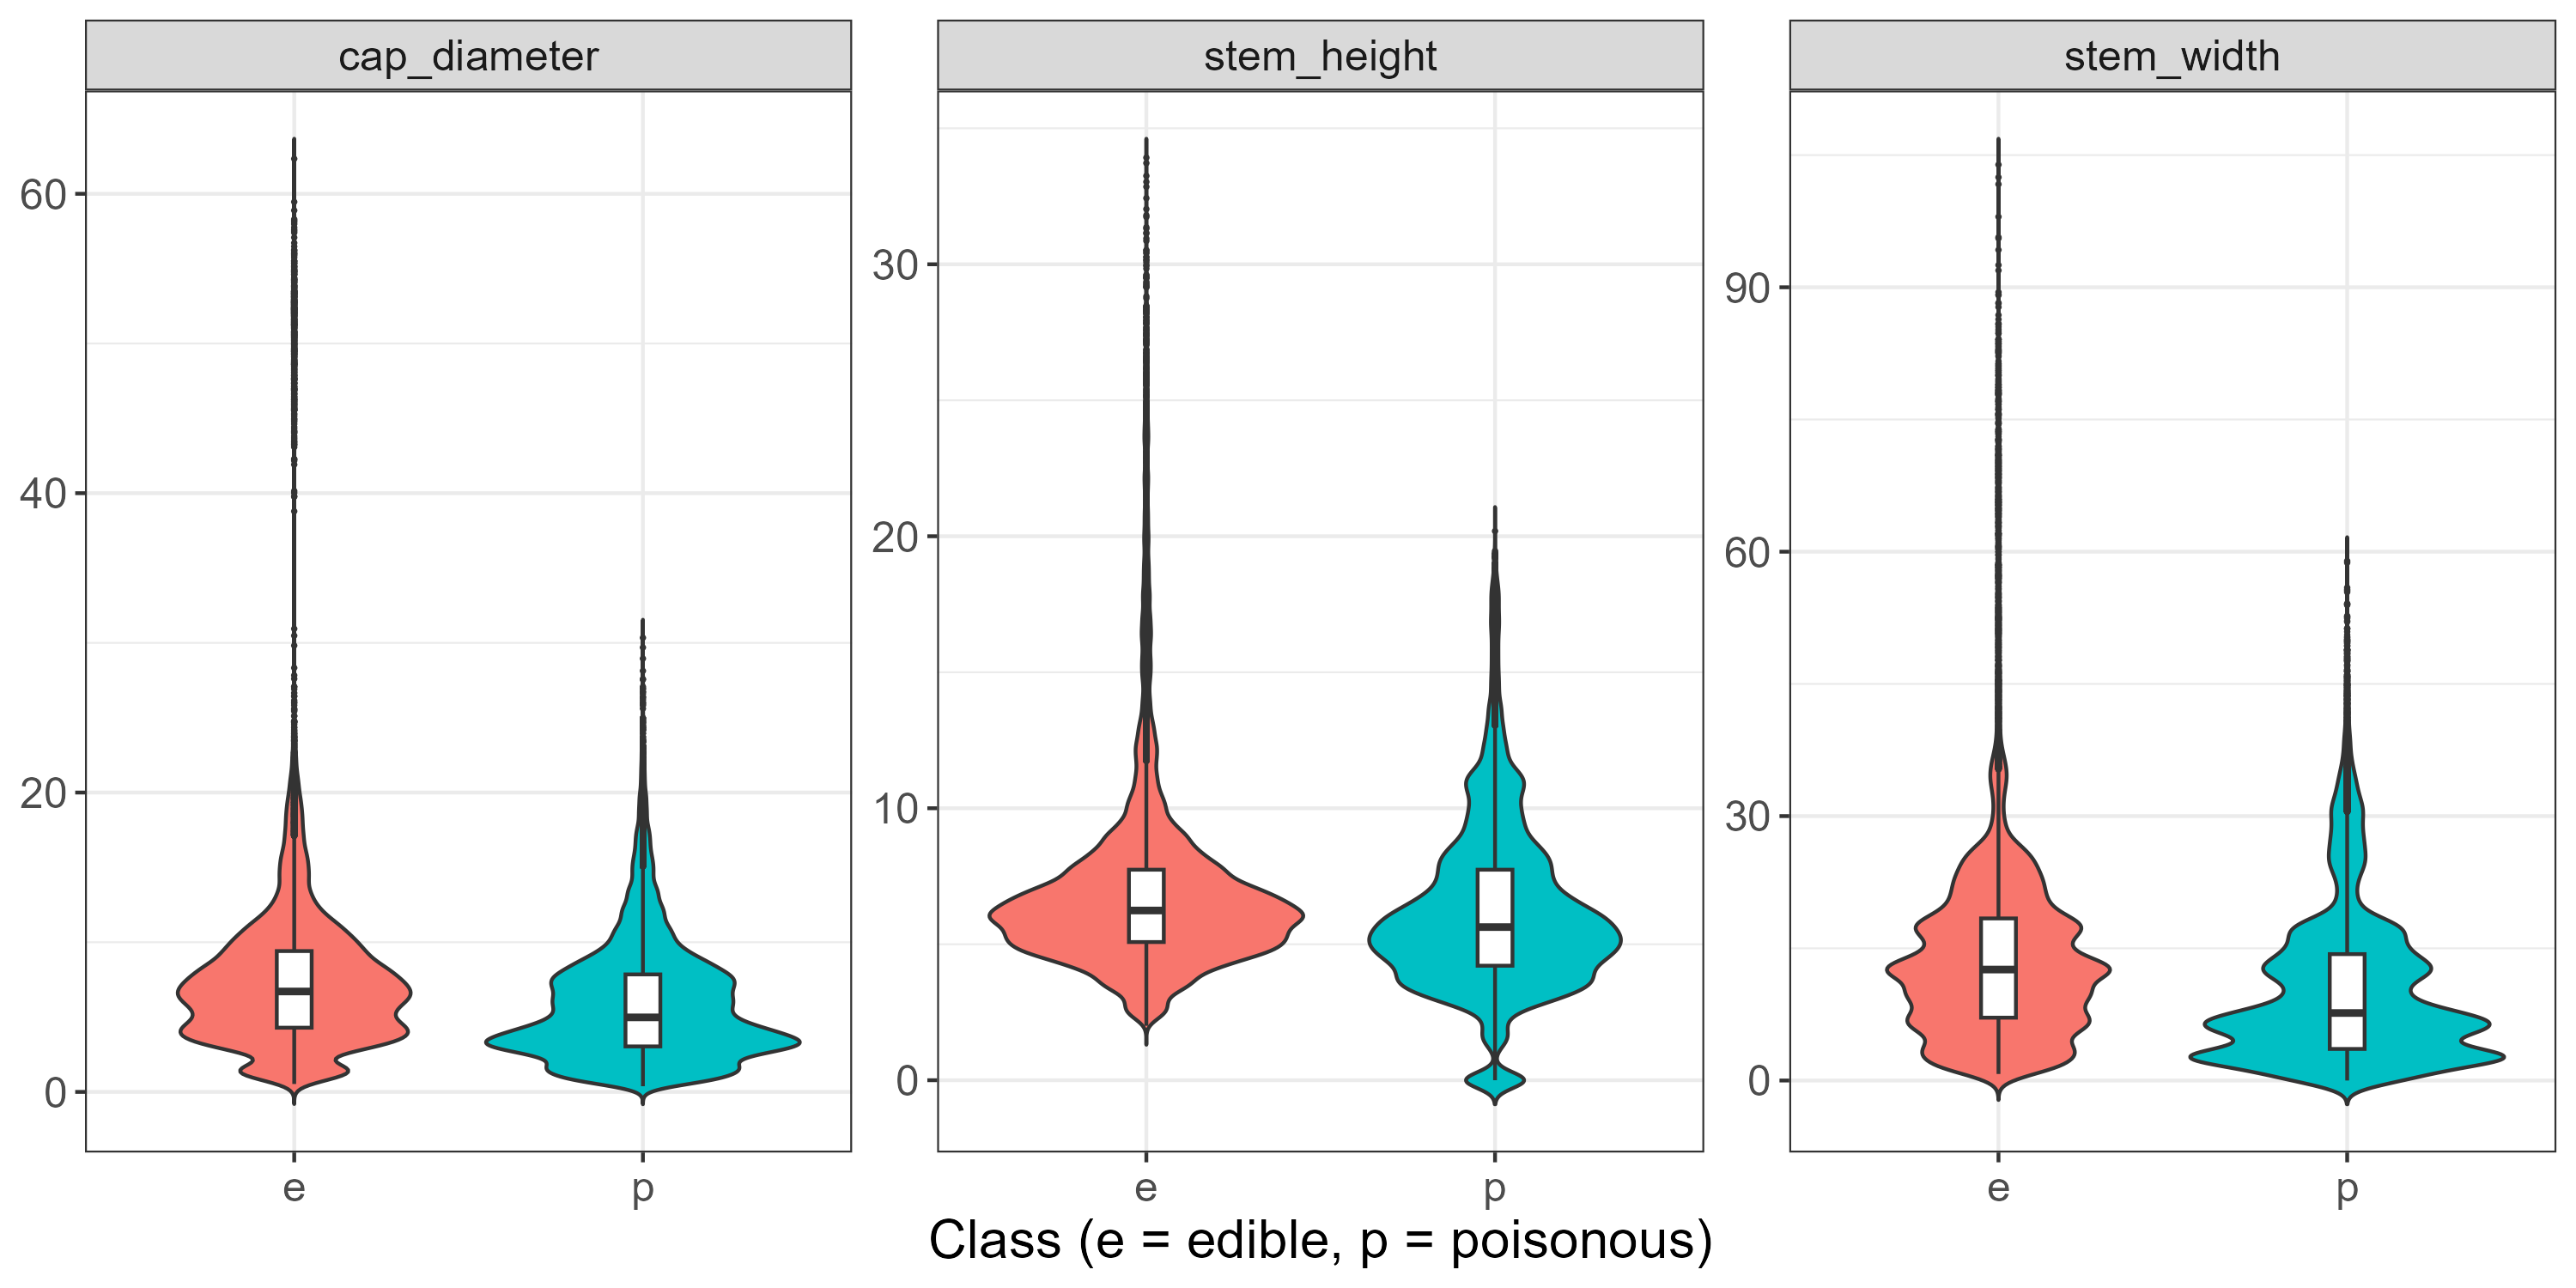
\includegraphics[width=0.95\textwidth]{Figure1-violin-plots.png}
\caption{Distribution of numeric features stratified by edibility class}
\label{fig:violin}
\end{figure}

The plots reveal several useful trends:
\begin{itemize}
  \item \textbf{Cap diameter} shows a wider spread in the edible class, with several outliers suggesting the presence of unusually large caps. Poisonous mushrooms, by contrast, tend to cluster within a narrower range.
  \item \textbf{Stem height} appears less distinctive between the two groups. While the edible class may have a slight skew toward taller stems, the overlap between the two distributions is substantial.
  \item \textbf{Stem width} exhibits the clearest separation. Edible mushrooms generally have thicker stems on average, making this variable a potentially strong predictor.
\end{itemize}

These observations hint that among the numerical features, \texttt{stem\_width} could provide the most useful information for classification, while the others may contribute indirectly through interactions or non-linear effects.

\subsection{Categorical Feature Distributions}

To assess how categorical variables vary with the class label, we created a set of count plots grouped by feature and colored by edibility class (Figures~\ref{fig:count} and~\ref{fig:countfull} in \ref{Appendix}).

\begin{figure}[h]
\centering
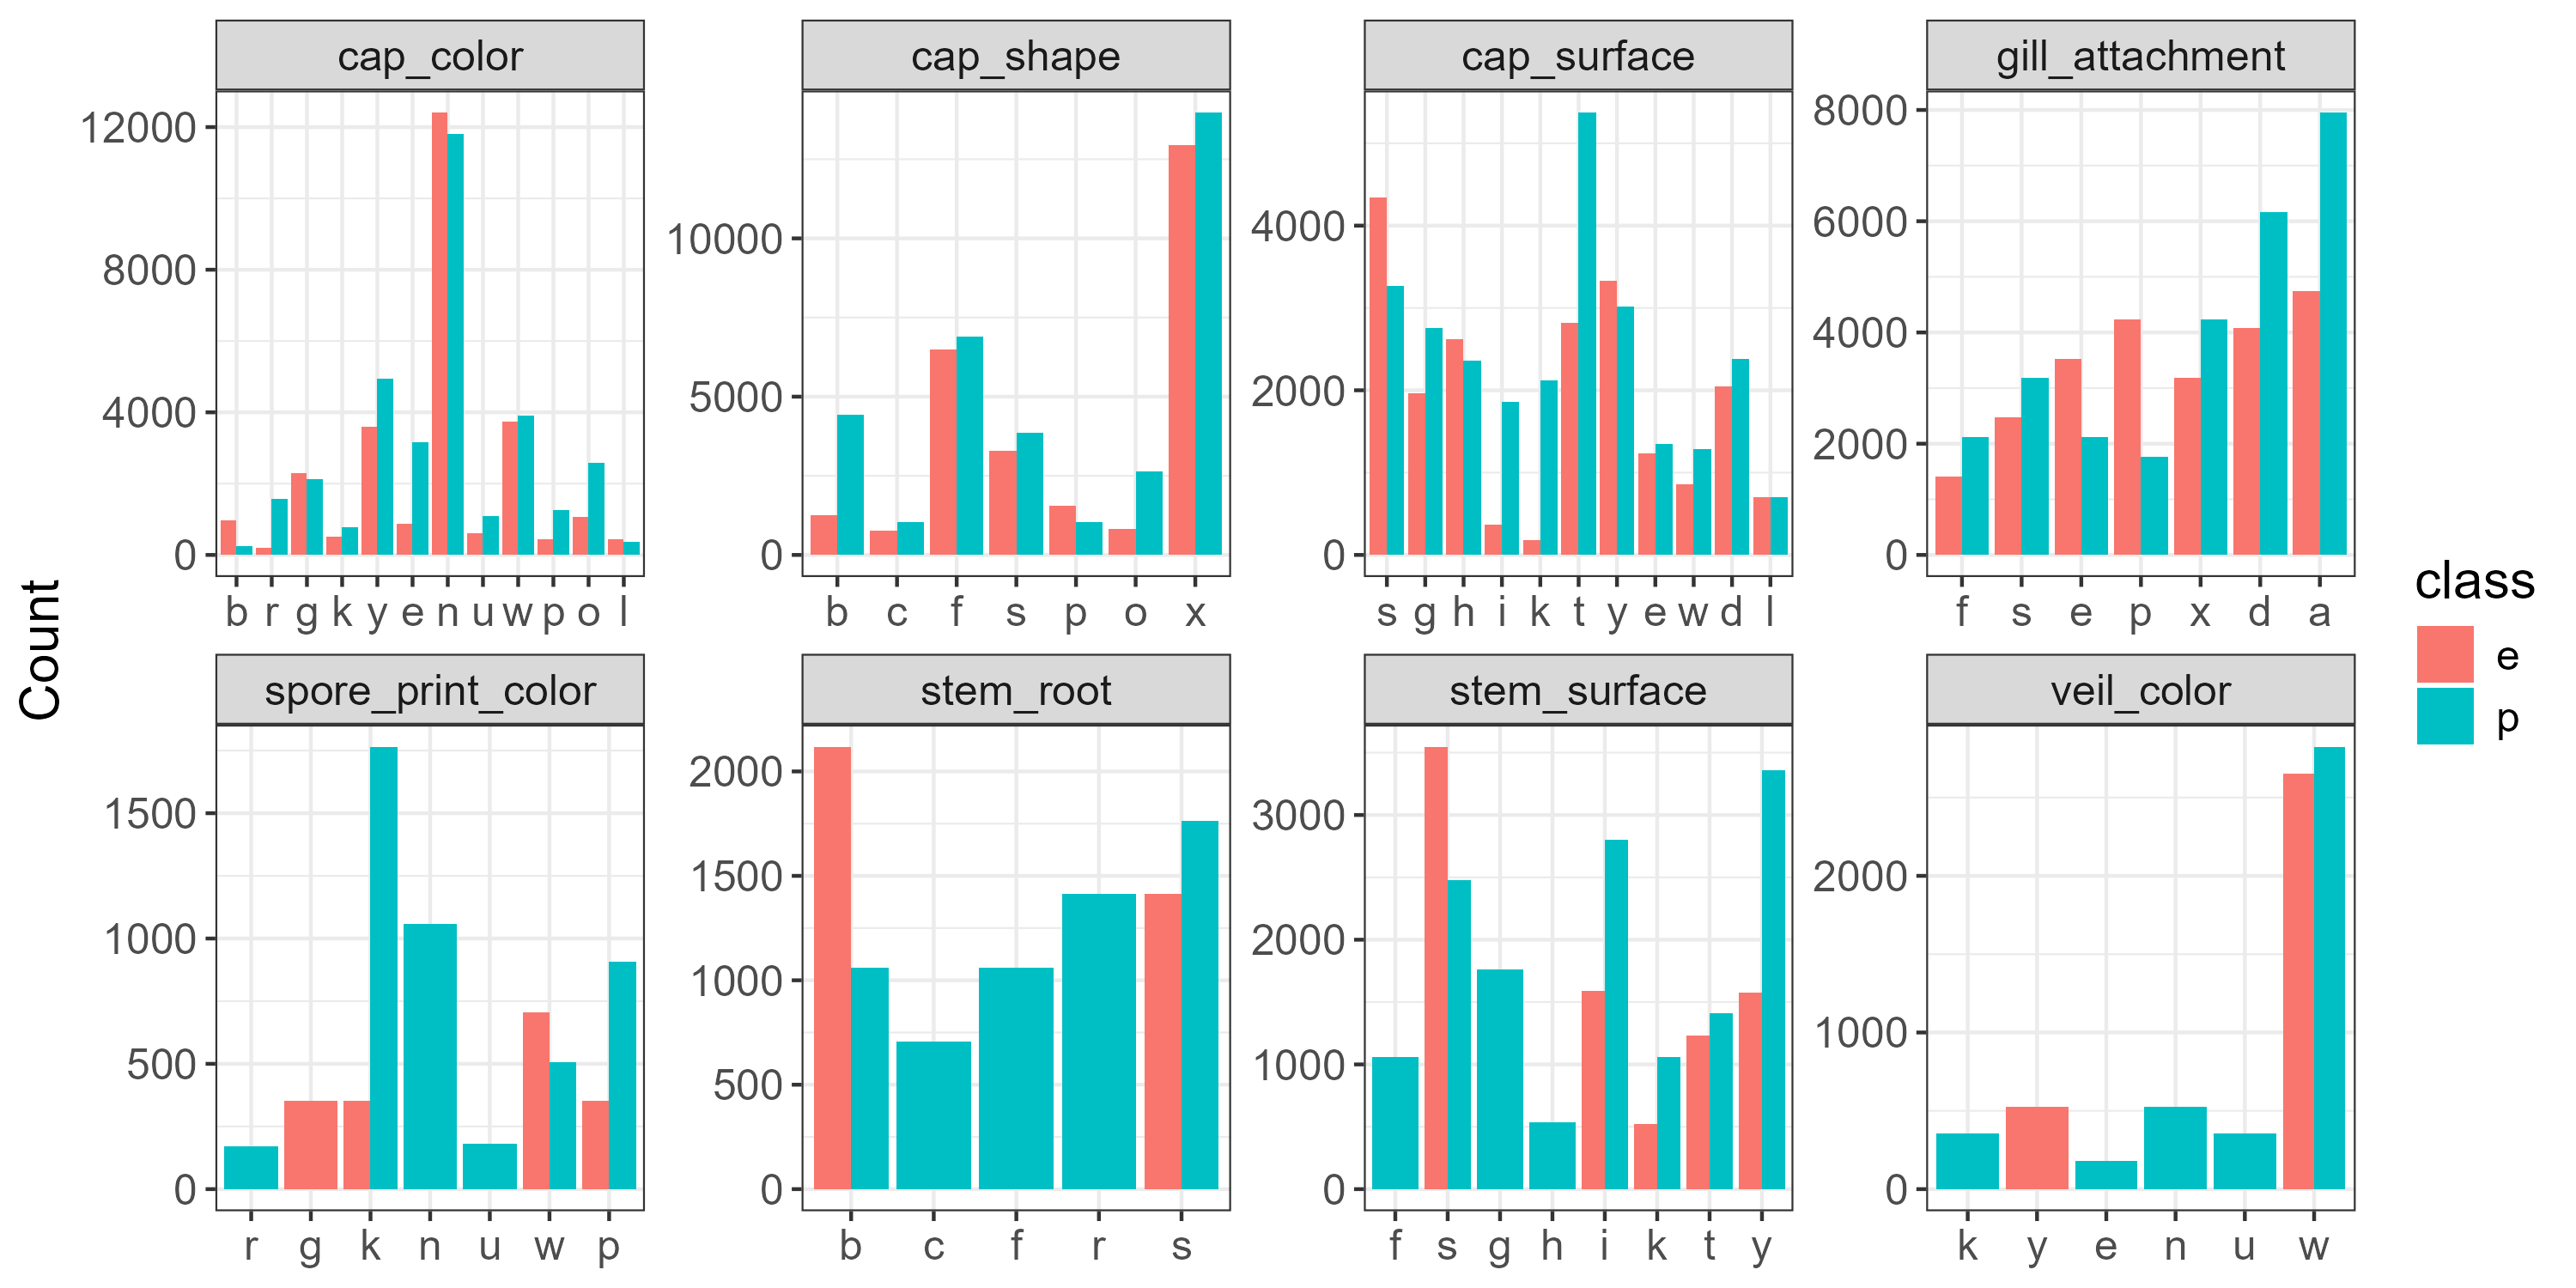
\includegraphics[width=0.95\textwidth]{Figure2-count-plots.png}
\caption{Class distribution for selected categorical features}
\label{fig:count}
\end{figure}

Several noteworthy patterns emerge:
\begin{itemize}
  \item Some feature values occur exclusively in one class. For example, certain \texttt{spore\_print\_color} values (e.g., \texttt{red}, \texttt{purple}) appear only in poisonous samples, while others (e.g., \texttt{gray}) are found solely in edible mushrooms.
  \item Other features, such as \texttt{cap\_surface} or \texttt{stem\_surface}, show skewed but not class-exclusive distributions, meaning they may still contribute predictive value when combined with other variables.
  \item A few features, like \texttt{veil\_type}, show little to no variability and may be uninformative or redundant.
\end{itemize}

Taken together, the exploratory analysis offers clear evidence that both numerical and categorical features contain meaningful information about the edibility label. This justifies the use of a flexible classifier like Random Forest, which can model both types of input without requiring heavy preprocessing.



\section{Chi-Squared Feature Evaluation}

To identify which categorical variables are most informative for predicting mushroom edibility, we applied a chi-squared test of independence. This statistical method evaluates whether the observed distribution of feature values differs significantly between edible and poisonous mushrooms. Features with larger chi-squared scores suggest a stronger class-association and are therefore more promising candidates for classification models.

The resulting feature importance scores are visualized in Figure~\ref{fig:chi}, where each bar represents a single feature’s total chi-squared score, ranked from weakest to strongest.

\begin{figure}[h]
\centering
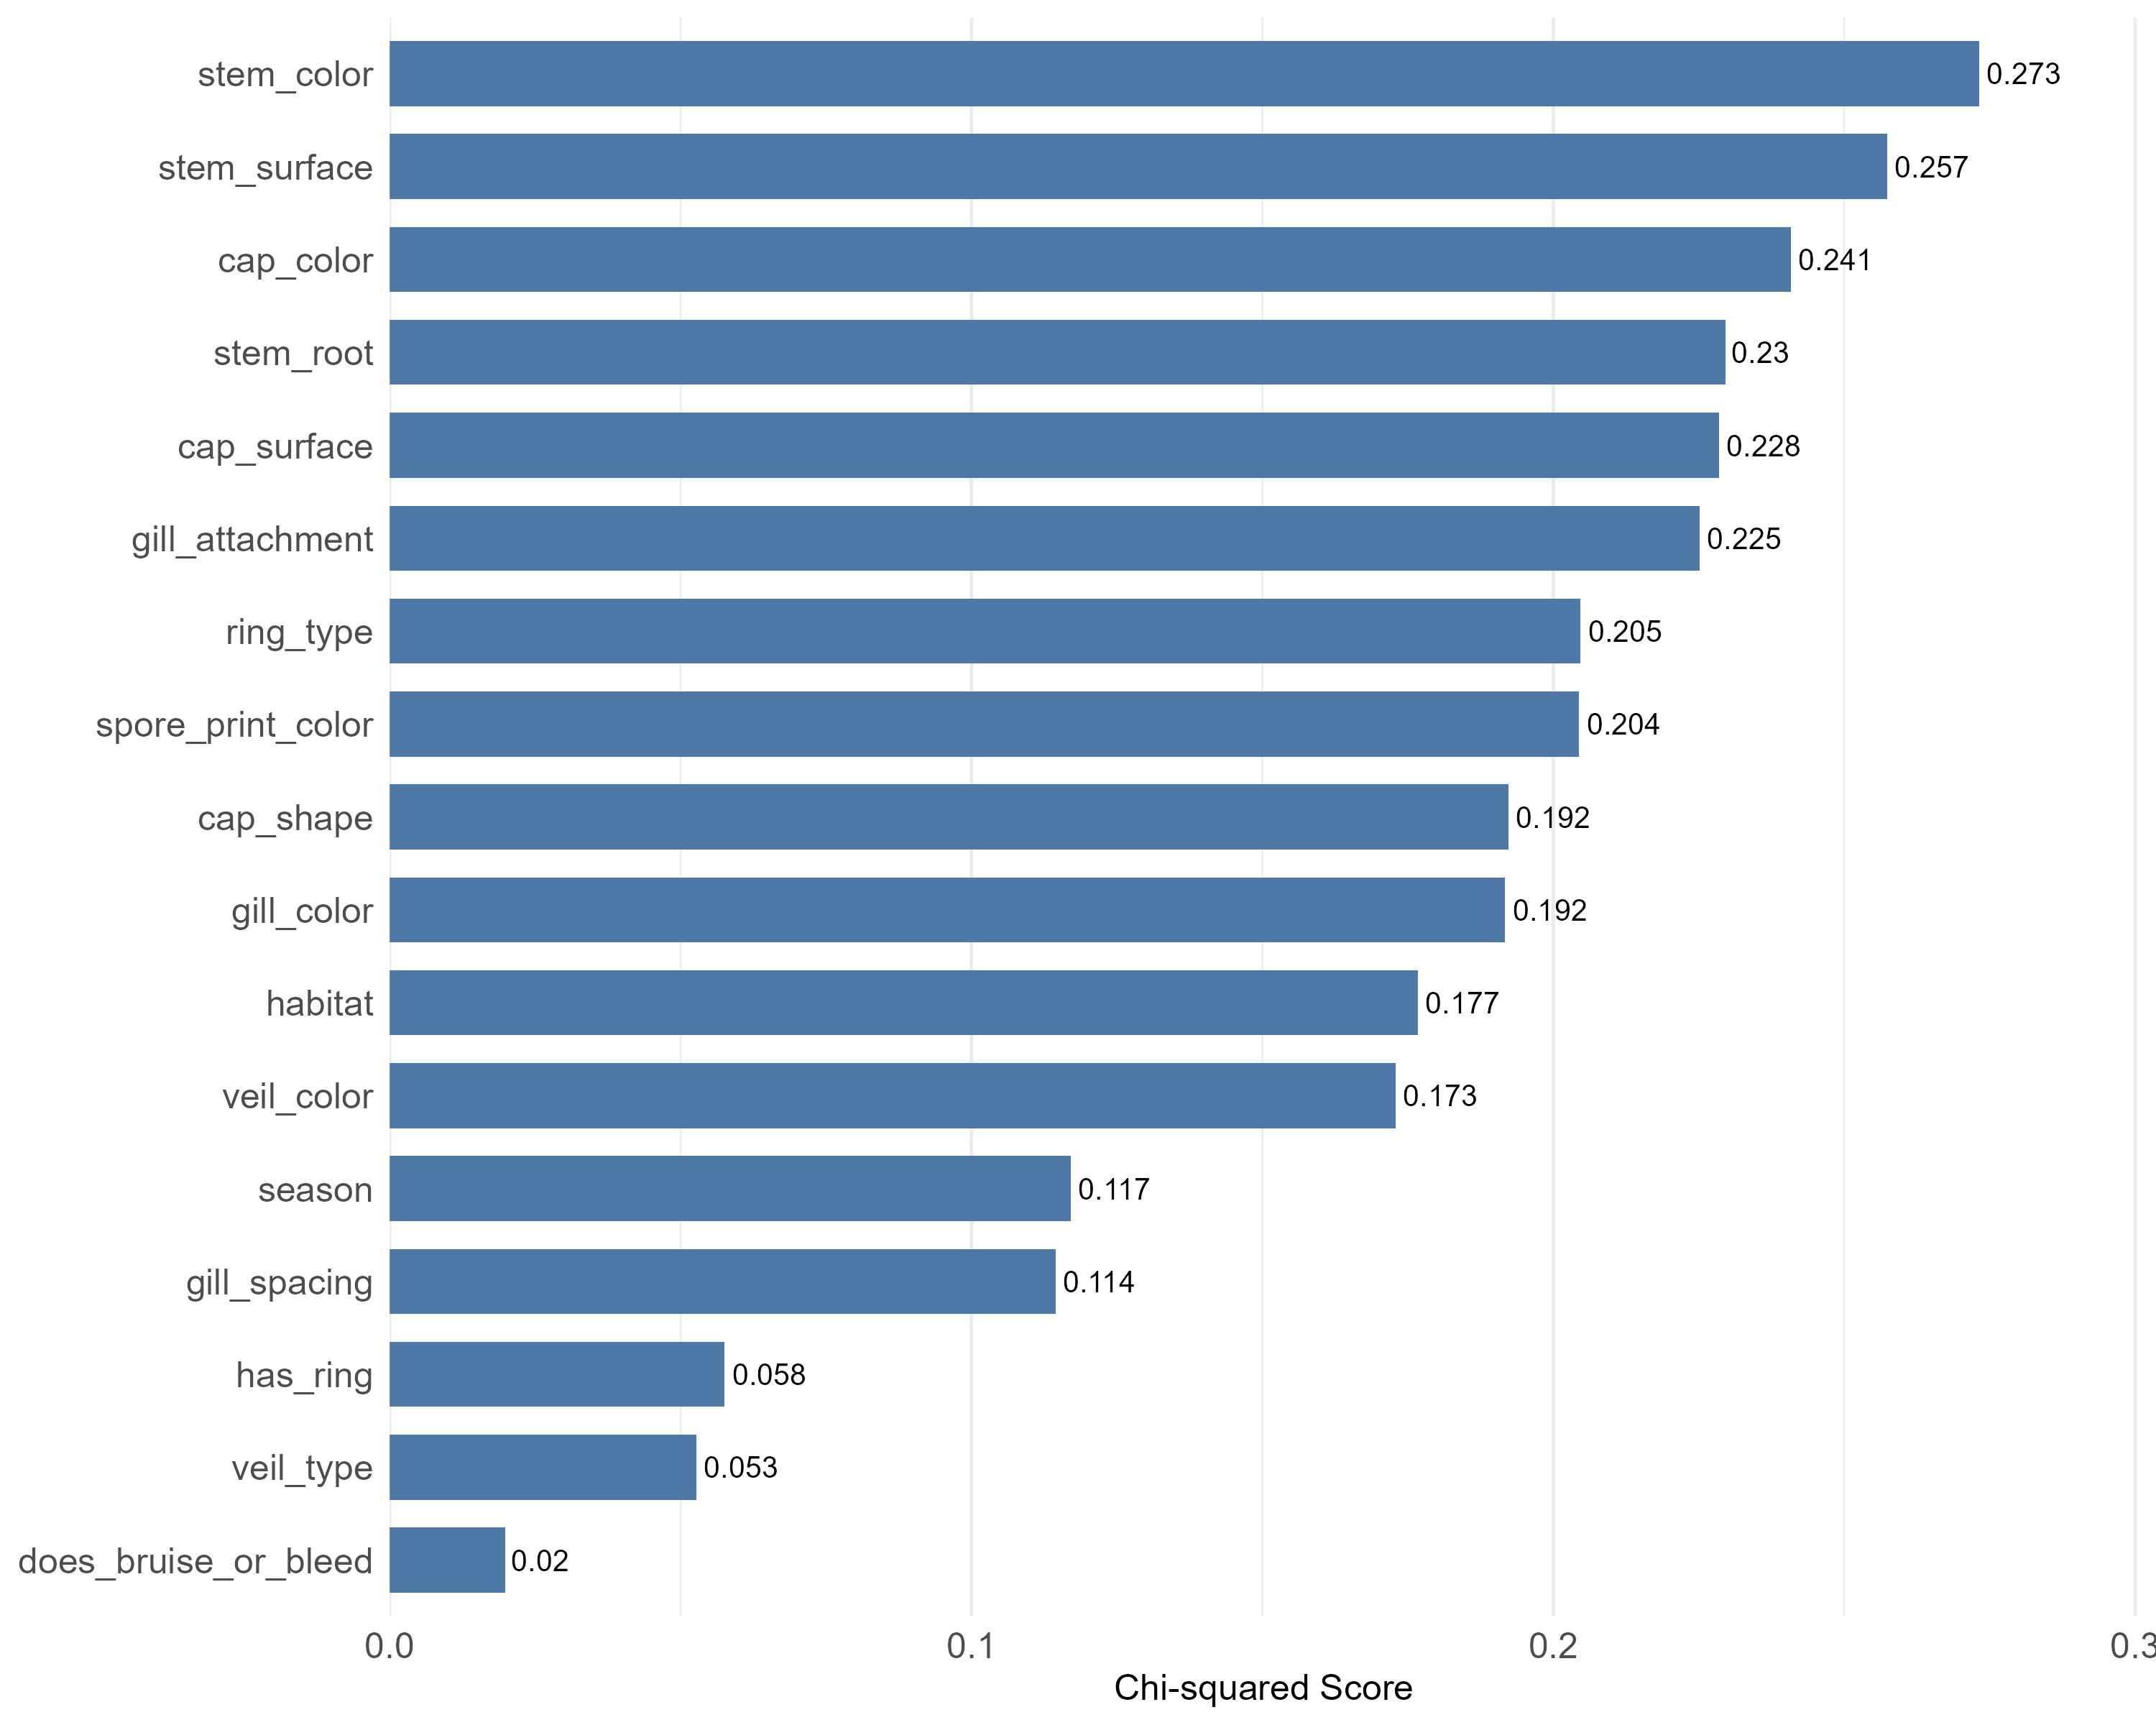
\includegraphics[width=0.95\textwidth]{Figure3-bar-chart.png}
\caption{Chi-squared scores for categorical features}
\label{fig:chi}
\end{figure}

Several observations emerge from this analysis:
\begin{itemize}
  \item Features such as \texttt{cap\_surface}, \texttt{gill\_attachment}, and \texttt{stem\_color} produced particularly high scores. This suggests a strong dependency between these features and the target class, consistent with what we saw in the count plots during exploratory analysis.
  \item Colors and surface textures\textemdash like those in \texttt{gill\_color} and \texttt{spore\_print\_color}\textemdash were also among the top features, reinforcing their potential predictive value.
  \item In contrast, some variables such as \texttt{veil\_type} and \texttt{habitat} had low scores, which may indicate minimal variation across classes or a limited role in determining edibility.
\end{itemize}

While chi-squared scores are useful for identifying statistically relevant features, they come with limitations. The test assumes independence between variables and does not consider possible interactions or non-linear relationships. As such, features with low individual scores might still contribute meaningfully to a model when used in combination with others\textemdash especially within ensemble algorithms like Random Forest.

This feature evaluation provides a data-driven justification for including or deprioritizing certain variables, and complements the qualitative insights gained during visual exploration.

\section{Random Forest Modeling}

\subsection{Model Evaluation Across Training Proportions}

To evaluate how the amount of training data affects classification performance, we trained Random Forest models using four different training set sizes: 1\%, 10\%, 30\%, and 70\% of the total dataset. The remaining data in each case was reserved for testing. For each configuration, we adjusted the number of trees (\texttt{ntree}) to achieve strong performance while keeping training time reasonable. The results are summarized in Table~\ref{tab:rf_accuracy}.

\begin{table}[h]
	\centering
	\begin{tabular}{|l|l|r|r|}
	\hline
	\textbf{Train Split} & \textbf{Test Split} & \textbf{ntree} & \textbf{Accuracy} \\
	\hline
	1\%   & 99\%  & 750 & 0.961114 \\
	10\%  & 90\%  & 330 & 0.999982 \\
	30\%  & 70\%  & 200 & 0.999977 \\
	70\%  & 30\%  & 100 & 1.000000 \\
	\hline
	\end{tabular}
	\caption{Random Forest accuracy under different train/test splits}
	\label{tab:rf_accuracy}
\end{table}

The results in Table~\ref{tab:rf_accuracy} show that the Random Forest classifier is remarkably resilient to variations in training size. Even when trained on just 10\% of the data, the model achieved accuracy above 99.99\%. At 70\% training data, the model perfectly classified all test examples. These outcomes suggest that the structure of the data is highly learnable and that the features contain strong class-separating information. 

Interestingly, even the smallest training scenario (1\%) yielded respectable performance, with an accuracy above 96\%. While this is lower than the other splits, it remains impressive given the limited number of training instances. Such results indicate that the model is not only accurate but also sample-efficient — an important trait for applications where labeled data may be scarce.

\begin{figure}[h]
\centering
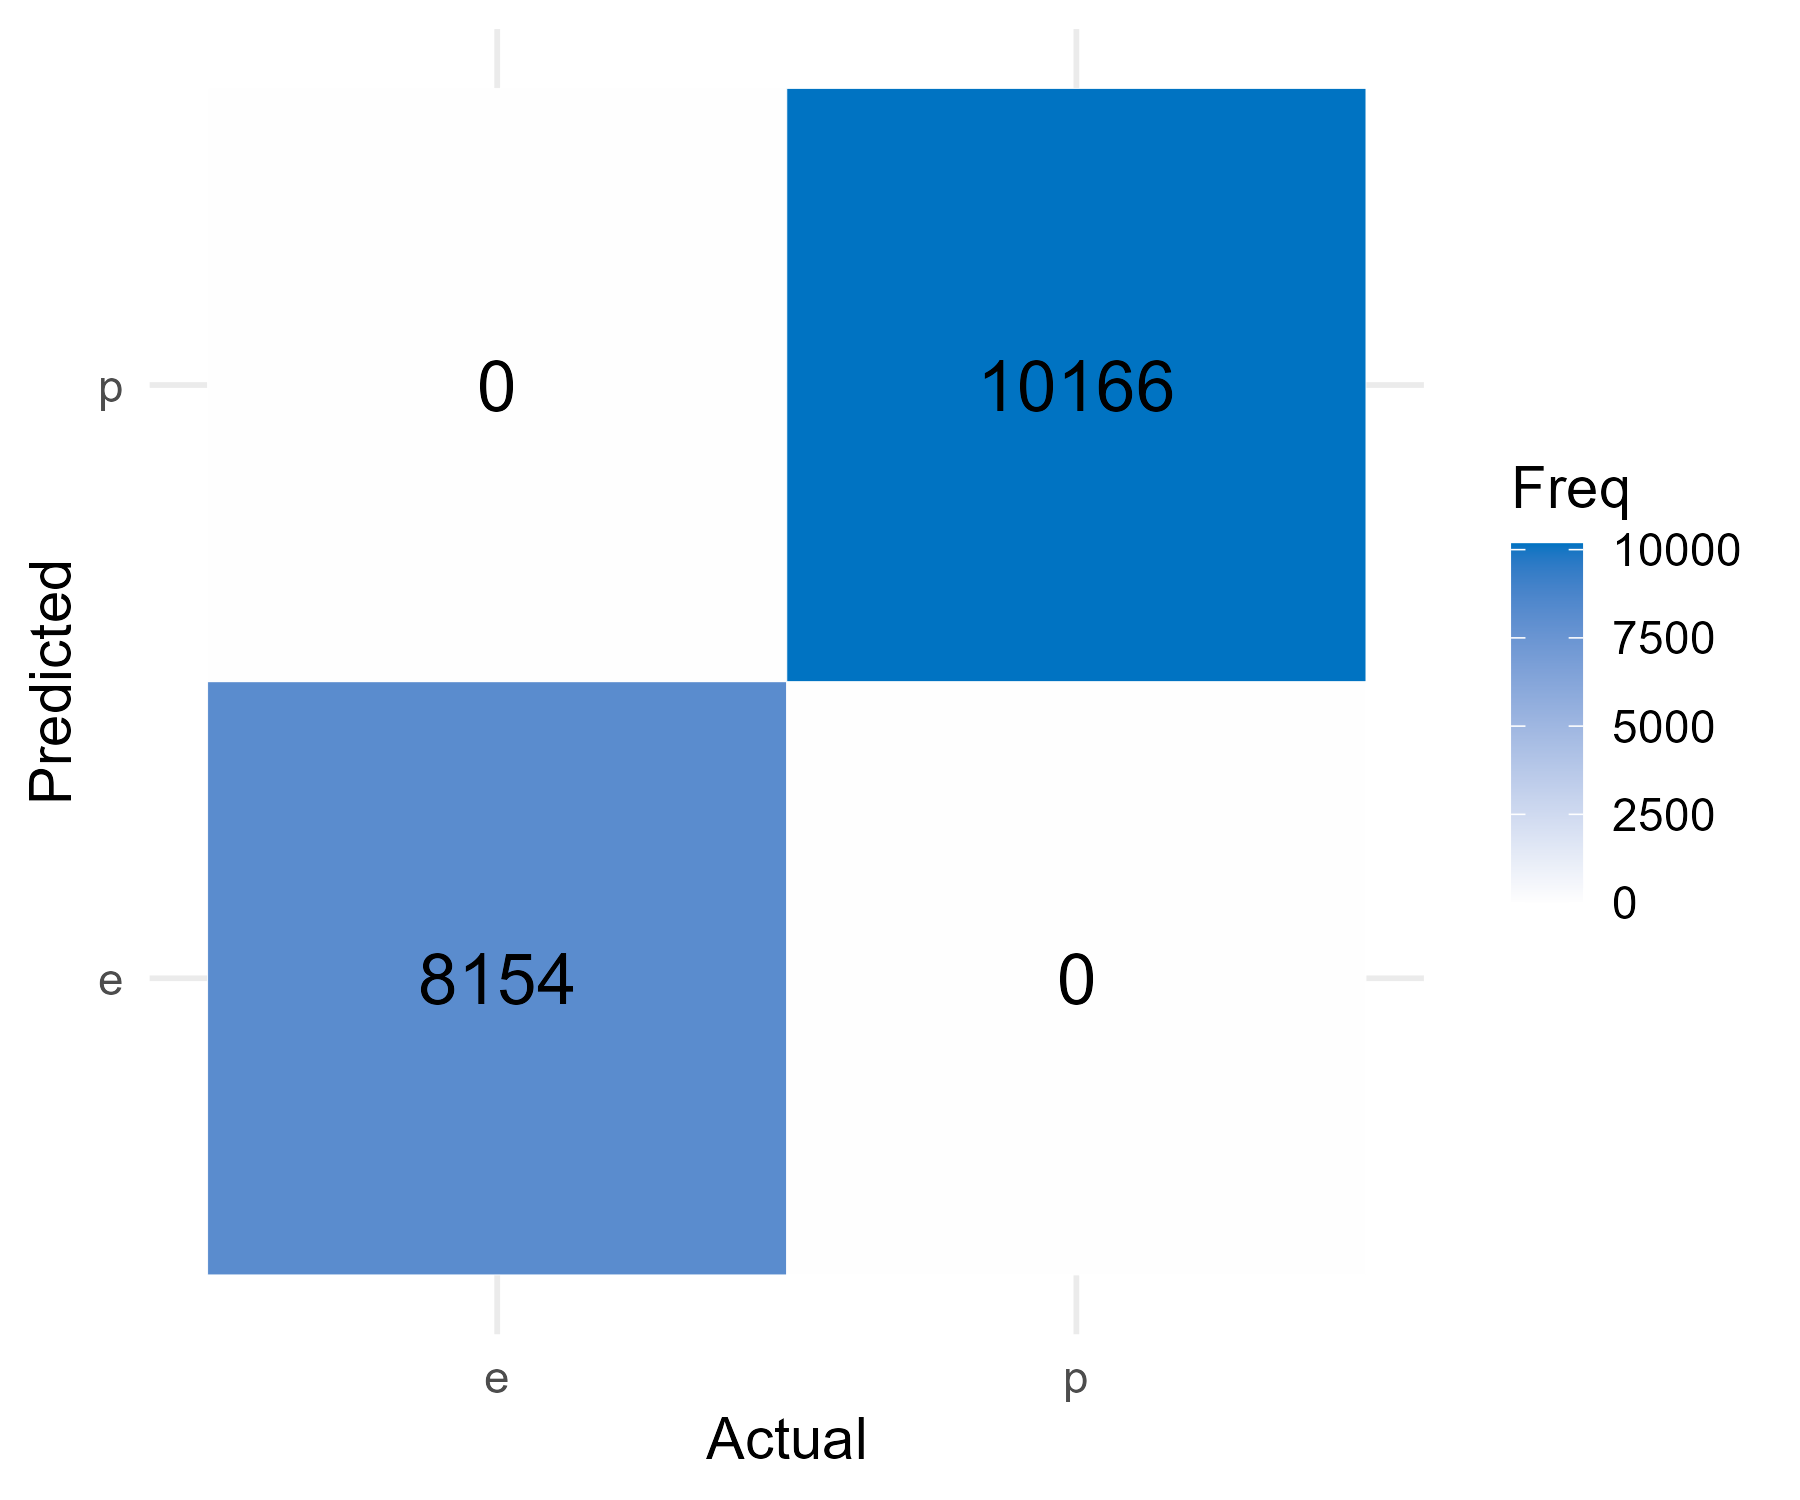
\includegraphics[width=0.6\textwidth]{Figure5-confusion-matrix.png}
\caption{Confusion matrix for the 70\% training split Random Forest model}
\label{fig:conf_matrix}
\end{figure}

To further support these accuracy metrics, we visualized the confusion matrix for the model trained on 70\% of the data, shown in Figure~\ref{fig:conf_matrix}. The matrix clearly shows a perfect separation of the two classes: no edible mushrooms were misclassified as poisonous, and no poisonous mushrooms were incorrectly labeled as edible. This reinforces the earlier numerical findings and offers additional reassurance that the model’s predictions are highly reliable. Moreover, the clean diagonal structure of the matrix indicates that the classifier is not overfitting or biased toward a particular class, even in the presence of some class imbalance.

\subsection{Feature Importance Analysis}

To gain insight into the factors driving classification performance, we extracted feature importance scores from the final Random Forest model trained on 70\% of the data. Figure~\ref{fig:gini} ranks each feature by its mean decrease in Gini impurity, which quantifies how much each variable reduces classification uncertainty within the ensemble.

\begin{figure}[h]
\centering
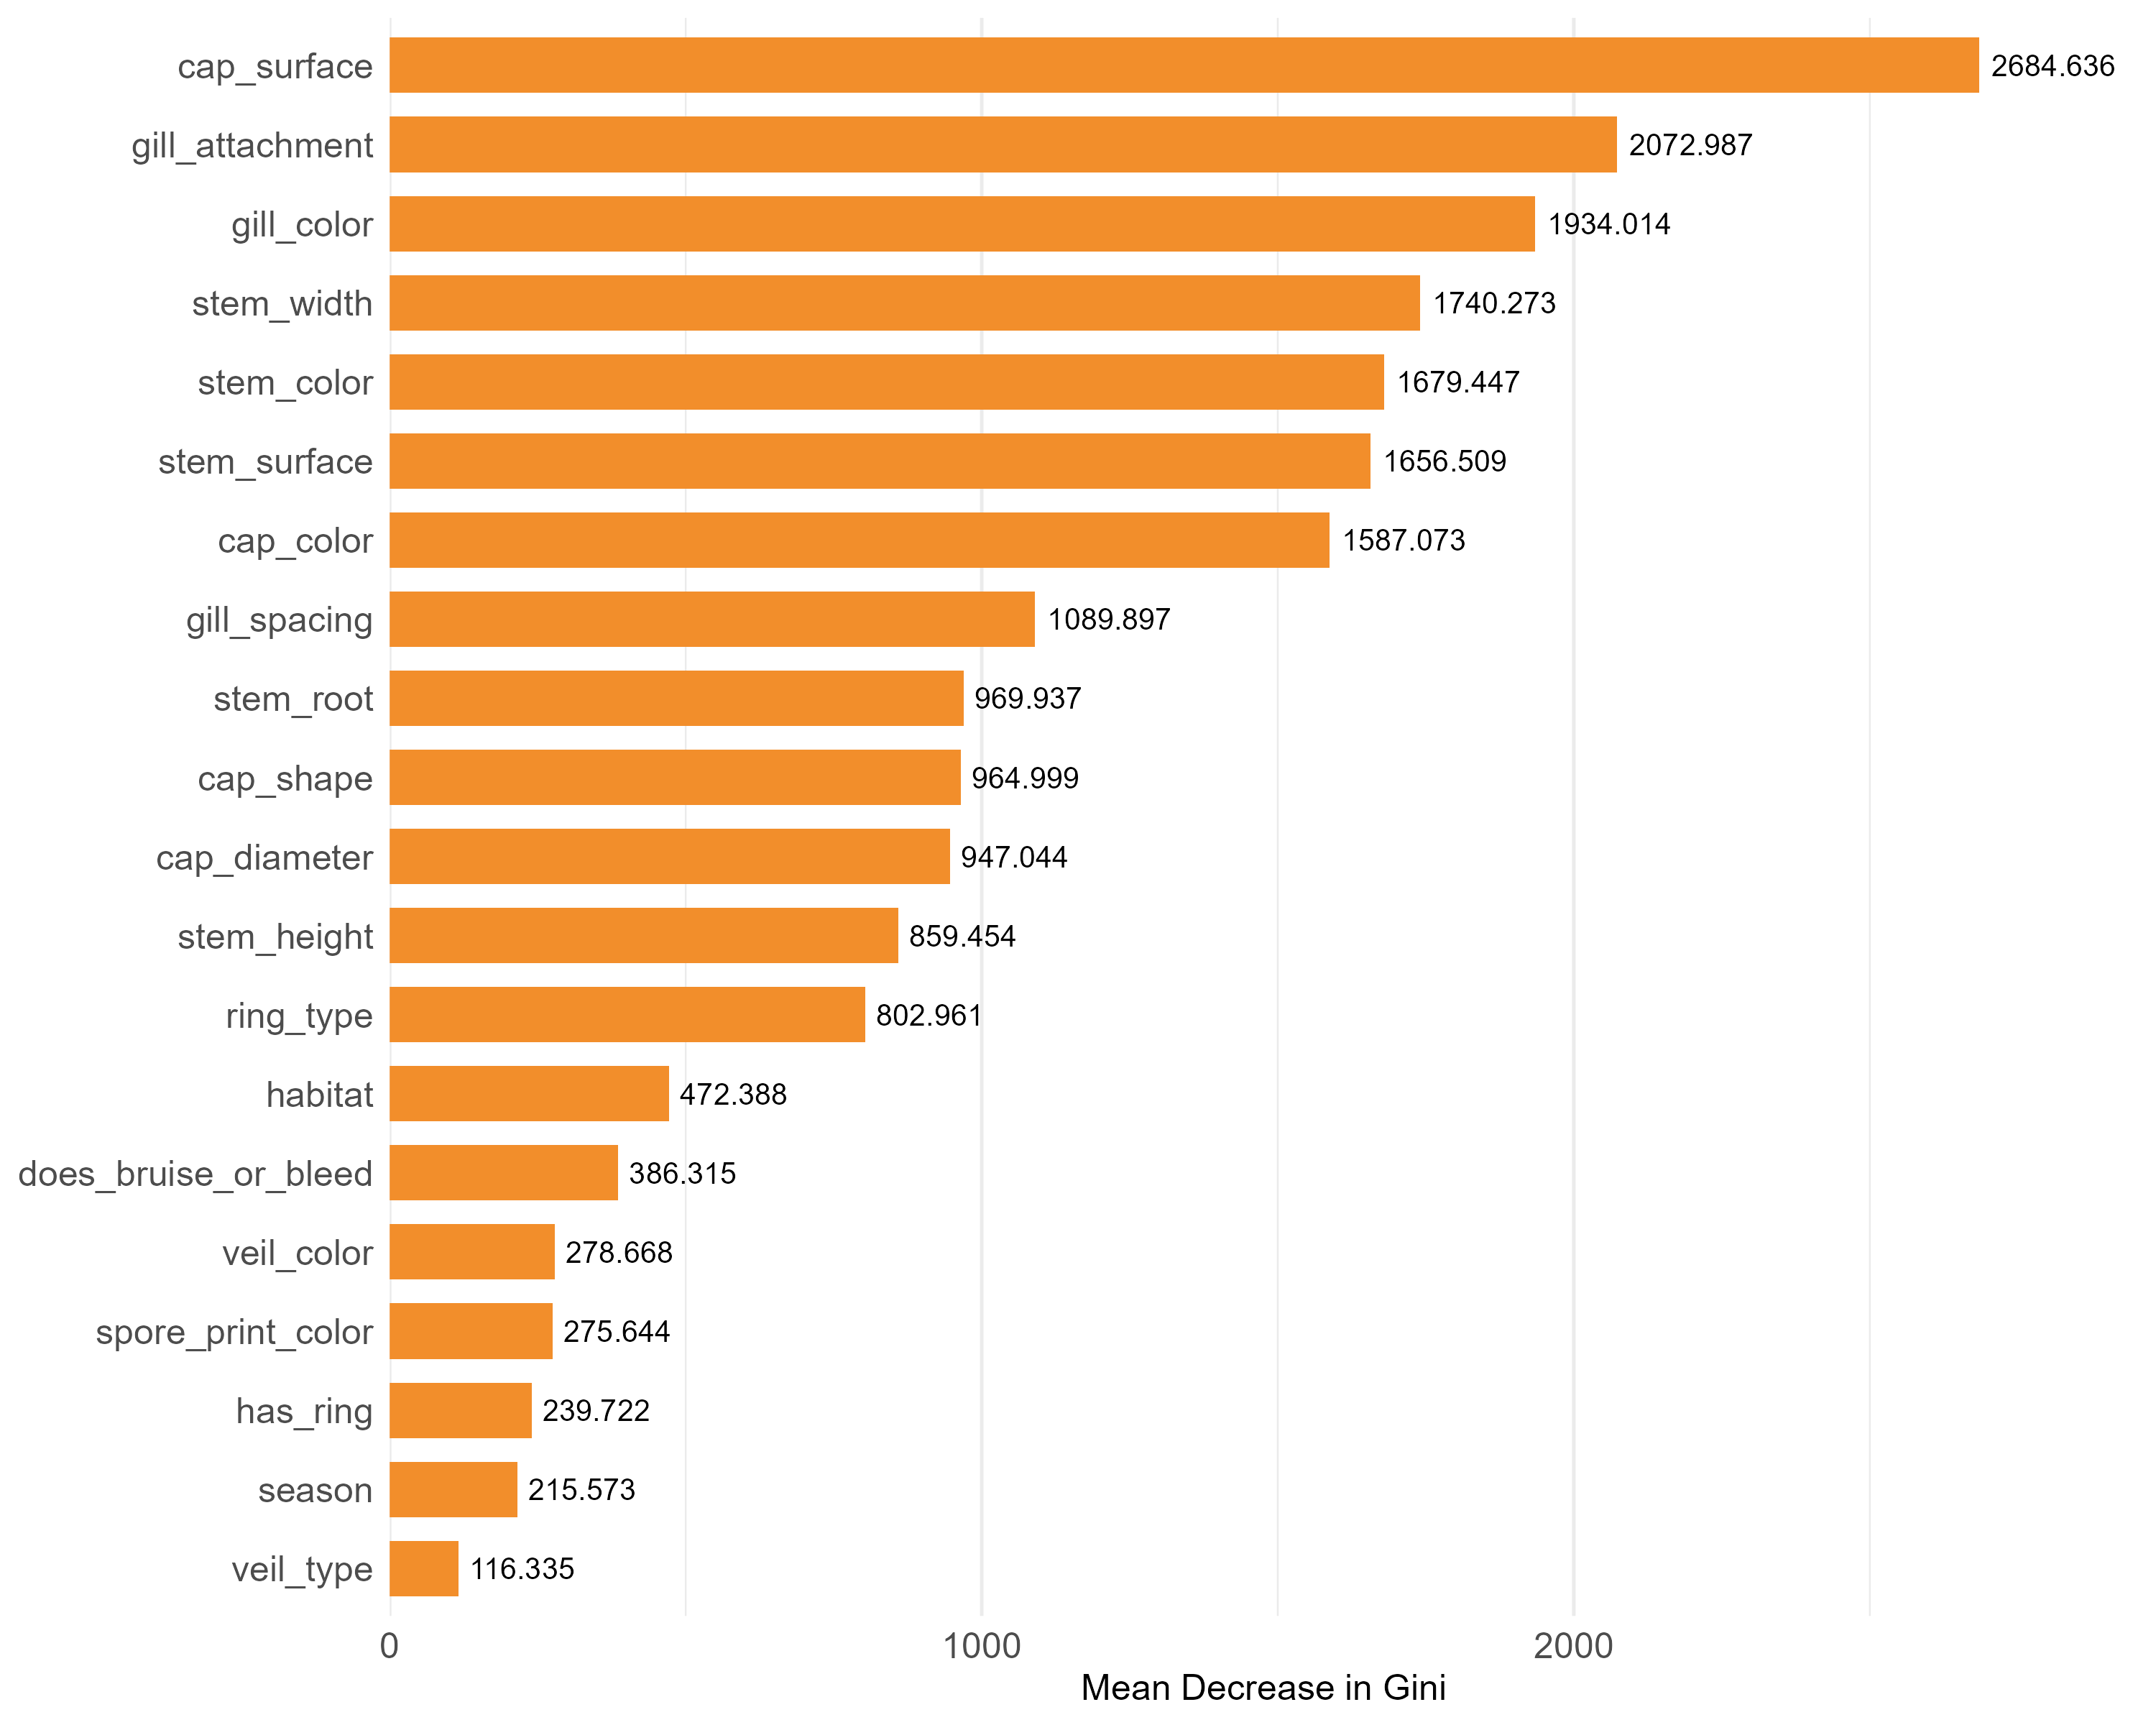
\includegraphics[width=0.95\textwidth]{Figure4-bar-chart-gini.png}
\caption{Random Forest feature importance (Gini)}
\label{fig:gini}
\end{figure}

Several trends emerge from this ranking:
\begin{itemize}
    \item Features such as \texttt{cap\_surface}, \texttt{gill\_attachment}, and \texttt{stem\_color} were consistently among the top contributors to model accuracy. These variables also showed strong associations in earlier visual and statistical analyses.
    \item Numerical features, particularly \texttt{stem\_width}, appeared prominently as well. This aligns with the violin plots where class-wise separation was most distinct for this attribute.
    \item Some variables that ranked low in the chi-squared test\textemdash such as \texttt{veil\_type}\textemdash also had minimal contribution here, providing cross-validation of their limited relevance.
\end{itemize}

Taken together, the feature importance analysis offers interpretability beyond model accuracy. It helps uncover which traits are biologically or visually most indicative of mushroom toxicity, which could be of use in real-world settings.

\section{Conclusion}

This replication study confirms and extends the findings of Brital et al.~\citep{brital2019edibility}, demonstrating that Random Forest remains a highly effective method for predicting mushroom edibility. Using a larger dataset and modern tools in R, we achieved near-perfect classification performance across a range of training scenarios.

Beyond performance metrics, we incorporated data visualization, statistical tests, and feature importance analysis to understand how different variables contribute to the model’s success. These steps improved both the interpretability and the robustness of our results.

While this replication focused on the Random Forest portion of the original work, it lays a foundation for further comparison with Bagging and Boosting, or for future studies using deep learning or ensemble stacking. Our pipeline is fully reproducible and publicly available, offering a reference point for similar classification tasks in food safety, biology, or pattern recognition.


\bibliography{bibliography}

\appendix 
\setcounter{section}{0}
\def\thesection{Appendix}
\section{}\label{Appendix}
\def\thesubsection{\Alph{subsection}}

\begin{figure}[h]
    \centering
    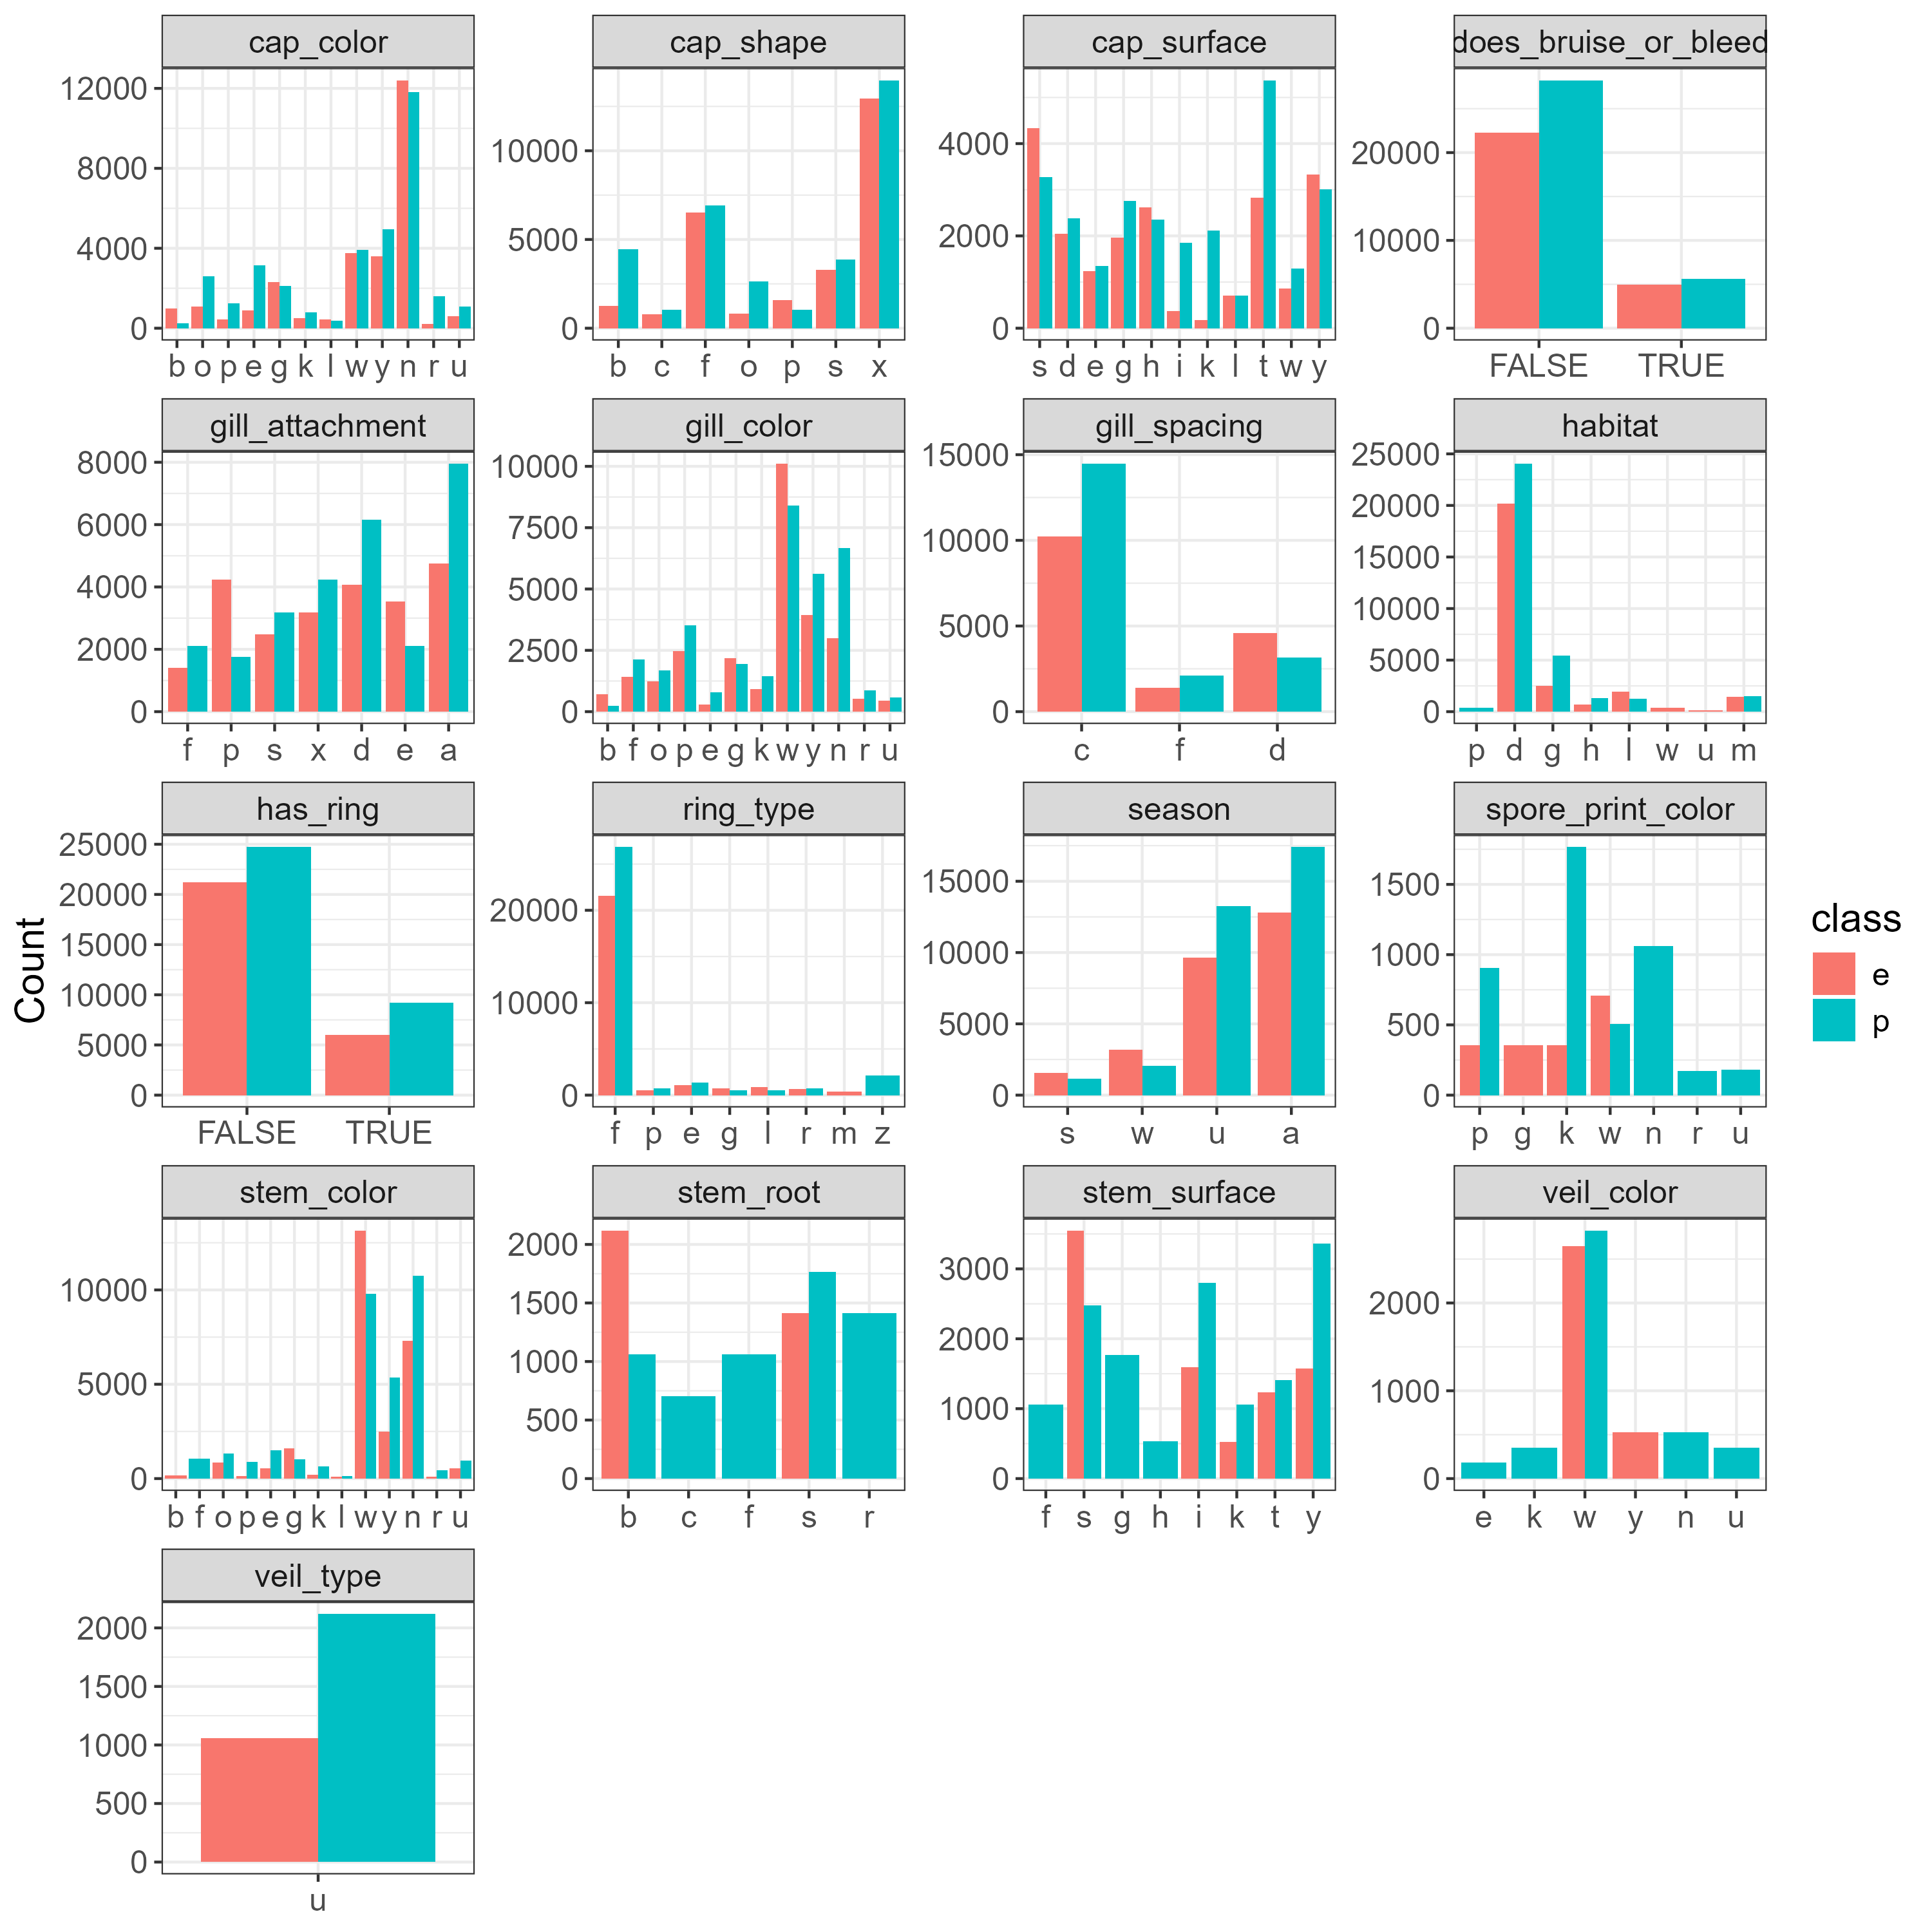
\includegraphics[width=1\textwidth]{Figure2.1-count-plots-full.png}
    \caption{Distribution of categorical features across class ('p'=poisonous, 'e'=edible)}
    \label{fig:countfull}
\end{figure}

Figure \ref{fig:countfull} is the countplots of all categorical features.

\end{document}